\documentclass[12pt,letterpaper]{article}           % fleqn: align equations left

% Document:
\usepackage{geometry}                                     % Custom margins for single page, etc.
\usepackage{fullpage}                                     % Use the full page
\usepackage{setspace}                                     % Enables custom margins, doublespacing, etc.
\usepackage{pdflscape}                                    % Use: \begin{landscape} ... \end{landscape}

% Font/text:
\usepackage[latin9]{inputenc}                             % Font definition and input type
\usepackage[T1]{fontenc}                                  % Font output type
\usepackage{lmodern}                                      % Latin Modern fonts
\usepackage{textcomp}   
\usepackage{multirow}                                  % Supports many additional symbols

%\usepackage[urw-garamond]{mathdesign} %dont use with amssymb, etc
%%%%Packages used without Mathdesign
\usepackage{amsmath}                                      % Math equations, etc.
\usepackage{amsthm}                                       % Math theorems, etc.
\usepackage{amsfonts}                                     % Math fonts (e.g. script fonts)
\usepackage{amssymb}                                      % Math symbols such as infinity
\DeclareMathOperator*{\Max}{Max}                          % Better looking max function
\DeclareMathOperator*{\Min}{Min}                          % Better looking min function

%%%%%%%%%%%%%%%%%%%%%%%5
\usepackage{xcolor}                                        % Enables colored text
\definecolor{darkblue}{rgb}{0.0,0.0,0.66}                 % Custom color: dark blue
\usepackage[hyperfootnotes=false,bookmarksopen]{hyperref} % Enable hyperlinks, expand menu subtree
\hypersetup{                                              % Custom hyperlink settings
    pdffitwindow=false,                                   % true: window fit to page when opened
    pdfstartview={XYZ null null 1.00},                    % Fits the default zoom of the page to 100%
    pdfnewwindow=true,                                    % Links in new window
    colorlinks=true,                                      % false: boxed links; true: colored links
    linkcolor=darkblue,                                   % Color of internal links
    citecolor=darkblue,                                   % Color of links to bibliography
    urlcolor=darkblue  }                                  % Color of external links

% Images:
\usepackage{graphicx}                                     % Allows .jpg images to be included
%\usepackage{epstopdf}                                    % Convert .eps images on the fly
%\usepackage{subfig}                                       % Enables arrayed images
\usepackage[section]{placeins}                            % Forces floats to stay in section
\usepackage{float}                                        % Used with restylefloat
\restylefloat{figure}                                     % "H" forces a figure to be "exactly here"
\usepackage[justification=centering]{caption}             % Center captions
\usepackage{subfig} %allow multiple floats in a figure



%\usepackage{datetime}                                     % Custom date format for date field
%\newdateformat{mydate}{\monthname[\THEMONTH] \THEYEAR}    % Defining month year date format
\usepackage{tikz}                                        % Timelines and other drawings
\usetikzlibrary{decorations}                             % Formating for Tikz
\usetikzlibrary{decorations.pathreplacing}
\usetikzlibrary{calc}
\usetikzlibrary{matrix}
\usetikzlibrary{positioning}
\definecolor{darkred}{rgb}{0.8,0,0}
\usepackage{tikz-3dplot}

\definecolor{red}{RGB}{213,94,0}


%%%%%%%%%%%MATH
\usepackage{graphicx}
\usepackage{caption}
%\usepackage{subcaption} %this produces an error with the package subfig

%Flow Chart
\tikzstyle{decision} = [diamond, draw, fill=blue!20, text width=4.5em, text badly centered, node distance=3cm, inner sep=0pt]
\tikzstyle{block}    = [rectangle, draw, fill=black!25, text width=5em, text centered, rounded corners, minimum height=4em]
\tikzstyle{line}     = [draw, -latex']
\tikzstyle{cloud}    = [draw, ellipse,fill=red!20, node distance=3cm, minimum height=2em]

\pagestyle{empty}

%%%%%%%%%%%%%%%%%%%%%%%%%%%%%%%5
\begin{document}



\begin{figure}[h]
	\begin{tikzpicture}[scale=.6]
	
	\draw[thick,<->] (0,10) node[above]{My Optimal Investment}--(0,0)--(10,0) node[right]{Partner's Investment};
	
	\node [below left] at (0,0) {$0$};
	
	\draw[style=dashed](0,0)--(9,9) node[above right]{$ 45^{\circ}$};
	
	%\draw(0,1) ..controls (6,2) and (6,8) .. (10,9) node[right]{$sf(k)$};
	\coordinate [] (A) at (0,1);
	
	\coordinate [] (B) at (3,2);
	\coordinate [] (C) at (4.5,5);
	\coordinate [] (D) at (6,7);
	\coordinate [] (E) at (10,8);
	
%	\draw[very thick,red] plot [smooth] coordinates { (A) (B) (C) (D) (E) };
%	
%	\node [below right] at (1,1) {Inefficient Equilibria};
%	\node [below right] at (7.5,7.5) {Efficient Equilibria};
	\end{tikzpicture}
\end{figure}

\newpage
$ $
\begin{figure}[h]
	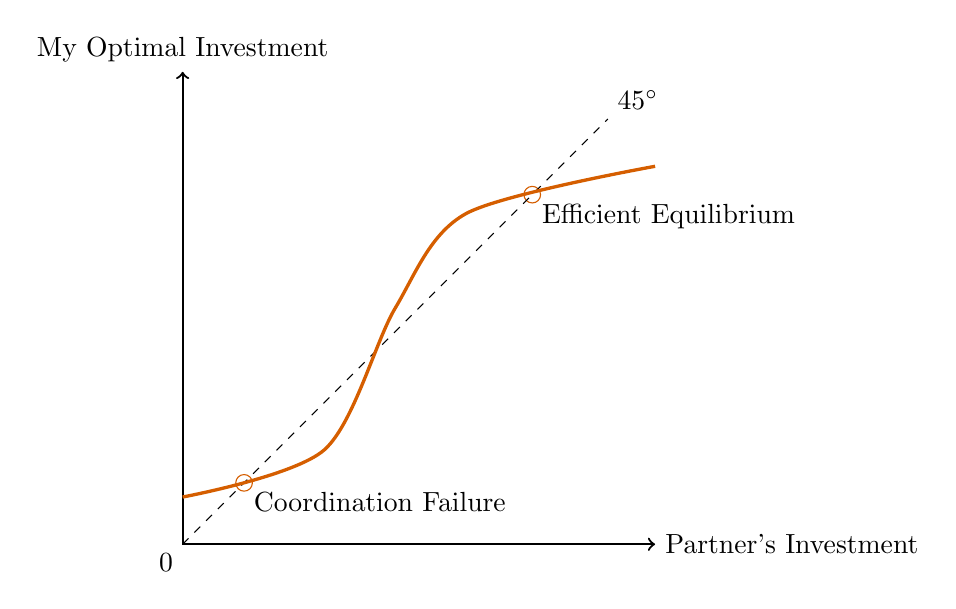
\begin{tikzpicture}[scale=.6]
	\draw [red,fill=white] (1.3,1.3) circle[radius= 0.5 em];
\draw [red,fill=white] (7.4,7.4) circle[radius= 0.5 em];
\node [below right] at (1.3,1.3) {Coordination Failure};
\node [below right] at (7.4,7.4) {Efficient Equilibrium};
	\draw[thick,<->] (0,10) node[above]{My Optimal Investment}--(0,0)--(10,0) node[right]{Partner's Investment};

	\node [below left] at (0,0) {$0$};
	
	\draw[style=dashed](0,0)--(9,9) node[above right]{$ 45^{\circ}$};
	
	%\draw(0,1) ..controls (6,2) and (6,8) .. (10,9) node[right]{$sf(k)$};
	\coordinate [] (A) at (0,1);
	
	\coordinate [] (B) at (3,2);
	\coordinate [] (C) at (4.5,5);
	\coordinate [] (D) at (6,7);
	\coordinate [] (E) at (10,8);
	
	\draw[very thick,red] plot [smooth] coordinates { (A) (B) (C) (D) (E) };

	\end{tikzpicture}
\end{figure}
\newpage
$ $
\begin{figure}[h]
	\begin{tikzpicture}[scale=.6]
	\draw [red,fill=white] (1.3,1.3) circle[radius= 0.5 em];
	\draw [red,fill=white] (7.4,7.4) circle[radius= 0.5 em];
	\node [below right] at (1.3,1.3) {Recession};
	\node [below right] at (7.4,7.4) {Expansion};
	\draw[thick,<->] (0,10) node[above]{My Optimal Investment}--(0,0)--(10,0) node[right]{Partner's Investment};
	
	\node [below left] at (0,0) {$0$};
	
	\draw[style=dashed](0,0)--(9,9) node[above right]{$ 45^{\circ}$};
	
	%\draw(0,1) ..controls (6,2) and (6,8) .. (10,9) node[right]{$sf(k)$};
	\coordinate [] (A) at (0,1);
	
	\coordinate [] (B) at (3,2);
	\coordinate [] (C) at (4.5,5);
	\coordinate [] (D) at (6,7);
	\coordinate [] (E) at (10,8);
	
	\draw[very thick,red] plot [smooth] coordinates { (A) (B) (C) (D) (E) };
	
	\end{tikzpicture}
\end{figure}

\newpage
$ $
\begin{figure}[h]
	\begin{tikzpicture}[scale=.6]
	\draw [red,fill=white] (1.3,1.3) circle[radius= 0.5 em];
	\draw [red,fill=white] (7.4,7.4) circle[radius= 0.5 em];
	\node [below right] at (1.3,1.3) {Poverty Trap};
	\node [below right] at (7.4,7.4) {High Income};
	\draw[thick,<->] (0,10) node[above]{My Optimal Investment}--(0,0)--(10,0) node[right]{Partner's Investment};
	
	\node [below left] at (0,0) {$0$};
	
	\draw[style=dashed](0,0)--(9,9) node[above right]{$ 45^{\circ}$};
	
	%\draw(0,1) ..controls (6,2) and (6,8) .. (10,9) node[right]{$sf(k)$};
	\coordinate [] (A) at (0,1);
	
	\coordinate [] (B) at (3,2);
	\coordinate [] (C) at (4.5,5);
	\coordinate [] (D) at (6,7);
	\coordinate [] (E) at (10,8);
	
	\draw[very thick,red] plot [smooth] coordinates { (A) (B) (C) (D) (E) };
	
	\end{tikzpicture}
\end{figure}

\newpage
$ $
\begin{figure}[h]
	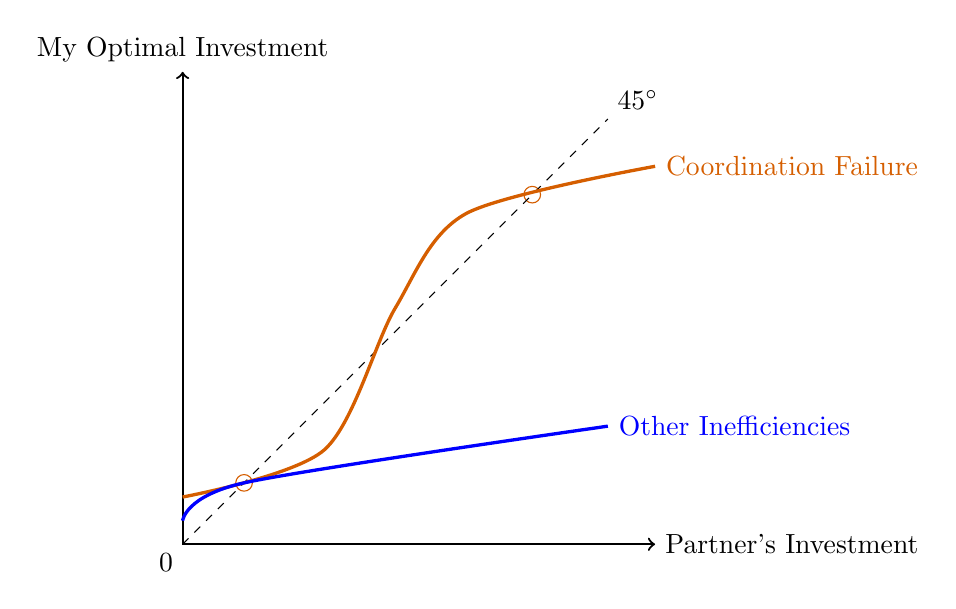
\begin{tikzpicture}[scale=.6]
	\draw [red,fill=white] (1.3,1.3) circle[radius= 0.5 em];
	\draw [red,fill=white] (7.4,7.4) circle[radius= 0.5 em];
%	\node [below right] at (1.3,1.3) {Poverty Trap};
%	\node [below right] at (7.4,7.4) {High Income};
	\draw[thick,<->] (0,10) node[above]{My Optimal Investment}--(0,0)--(10,0) node[right]{Partner's Investment};
	
	\node [below left] at (0,0) {$0$};
	
	\draw[style=dashed](0,0)--(9,9) node[above right]{$ 45^{\circ}$};
	
	%\draw(0,1) ..controls (6,2) and (6,8) .. (10,9) node[right]{$sf(k)$};
	\coordinate [] (A) at (0,1);
	
	\coordinate [] (B) at (3,2);
	\coordinate [] (C) at (4.5,5);
	\coordinate [] (D) at (6,7);
	\coordinate [] (E) at (10,8);
	
	\coordinate [] (AA) at (0,.5);
	\coordinate [] (BB) at (1.3,1.3);
	\coordinate [] (CC) at (9,2.5);
	\draw[very thick,red] plot [smooth] coordinates { (A) (B) (C) (D) (E) }node[right]{Coordination Failure};
	
	\draw[very thick,blue] plot [smooth] coordinates { (AA) (BB) (CC)}node[right]{Other Inefficiencies};
	
	\end{tikzpicture}
\end{figure}

\end{document}
